\chapter{Sample First Chapter\label{chap1}}


\section{Introduction}

I wouldn't actually name any of my chapter files chapter1.tex,
chapter2.tex, etc. 
   You might decide to swap them around at some
point, and then things can get messy, especially if you've labeled
things inside those files with labels like ``chap1.''  Computers
are good at counting things, let \LaTeX\ do that for you.  Be general
with your naming scheme, you can always rearrange things by altering
their order in the main dissertation.tex file.\footnote{Look at me!  I'm a footnote!}.


\section{Math Example\label{math}}

This is a real short example of using the equation environment.

\begin{equation}
	y = mx + b
\end{equation}

There is an awful lot that the equation environment and math mode
can do for you.


\section{How to cite your references\label{ref_citation}}

Here is an example of references using the natbib package and
`uabibnat.bst' file.  You can reference in a number of ways.  The
ones that are most useful are parenthetical \citep{article,articletwo}
or inline, as in \citet{articletwo} said this or that.  You can
also include information within the citation \citep[e.g.][doesn't
have any page numbers]{2003jgr}.  You don't even need to have the
reference in your text to be included.  \nocite{2004LPI}

For other ways of referencing, you can read more about the natbib
package by reading its documentation.  You should be able to find
the DVI file on your system where natbib was installed.  On my
system it's at /usr/local/share/texmf/doc/latex/natbib/natbib.dvi.


\section{Graphics\label{graphics}}

On the next page is a figure inclusion using the `graphicx' package.
This puts figures on their own page by themselves.  They don't need
to be on separate pages, there is no requirement that they be on
separate pages.  If you want to put a figure on a page with text,
don't include the \emph{p!} option in square brackets at the begin
figure command (as I have commented out below).

Also note that the \verb=\caption= command has an optional
square-bracketed argument and a curly-bracketed argument.  Whatever
you put in square brackets will be used as the short caption, and
will go into the List of Figures.  The stuff in the curly brackets
will be placed on the page under your figure.

% \begin{figure}
\begin{figure}[p!]
\begin{center}
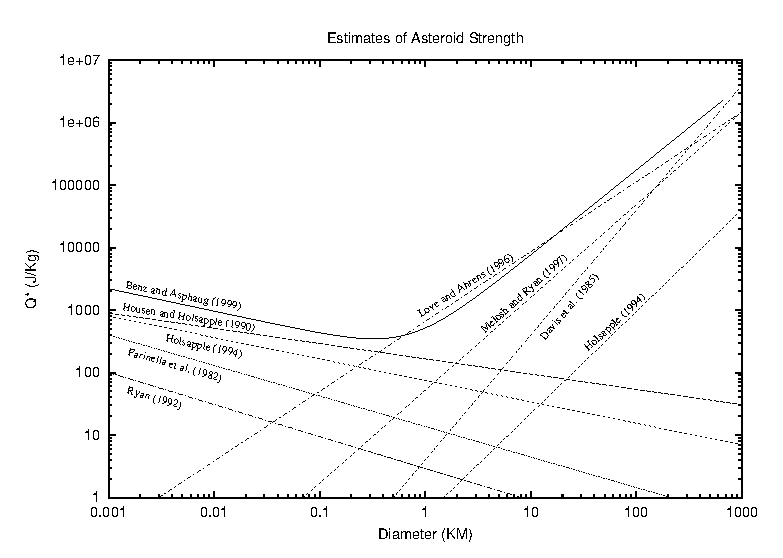
\includegraphics{figure.eps}
\caption[Short figure caption for LOF]{Sample figure caption (to appear below
the actual figure). \label{samplefig}}
\end{center}
\end{figure}

